\section{Realization}
\label{realisation}

Our implementation of the plug-in corresponds to the schema presented in the Figure \ref{flowchart}. We can divide our work into 2 stages; first we analyze and model the Android Intents and then develop this model into abstract and concrete syntax. The second stage is the plug-in development where we transform our existing abstract syntax data into structured JDT methods which will be called to perform our code generation. All the steps will be described in more details in this section.  

\begin{figure}[t]
\begin{minipage}{0.5\textwidth}
\label{flowchart}
  \centering
    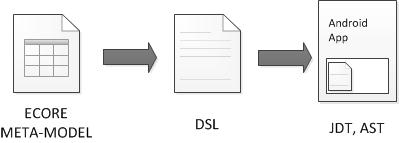
\includegraphics[width=.95\textwidth]{flowchart}
  \caption{Flow chart}
\end{minipage}%
\begin{minipage}{0.5\textwidth}
\label{asttreeview}
  \centering
    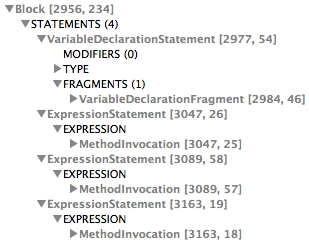
\includegraphics[width=.95\textwidth]{ast}
  \caption{AST of Intent Code}
\end{minipage}%
\end{figure}

We begin by determining the DSL of Android Intents and built our Ecore meta-model which reflected the DSL. Our DSL is based on several examples taken from Open Intents website\footnote{http://www.openintents.org/en/}, the default Android Intents included in Android, and finally the knowledge presented in the chapter \ref{intents}. The final Ecore model is shown the Figure \ref{meta-model}.

\begin{figure}[t]
\label{meta-model}
  \centering
    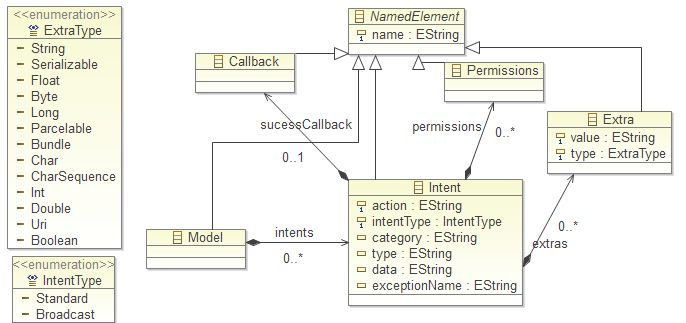
\includegraphics[width=0.9\textwidth]{metamodel}
  \caption{Meta-model of Intent}
\end{figure}

The second stage of development was to take this model and build the Xtext grammar. The final Xtext grammar we produced was based on the default grammar that was generated but with several modifications for simplification and the use of enumerated types. To test the grammar we developed several models based on some examples that we had previously chosen. This allowed us to make changes to both the Xtext grammar and the Ecore model when one or both did not suit the required data from the Intents. The developed models in our DSL are used as our dataset for the plug-in. An example of an Intent in our DSL is shown in the Listing \ref{dsl}.

{\footnotesize\begin{lstlisting}[escapechar=!,label=dsl,caption=Intent in DSL]
ImplicitIntent ActionSendText {
	type "text/plain"
	category "android.intent.category.DEFAULT"
	action "android.intent.action.SEND"
	extras {
		StringExtra "android.intent.extra.TEXT" !$\hookleftarrow$!
		"Put your text here"
	}
},
\end{lstlisting}}

The plug-in uses Model-to-Model transformations, and for this purpose we use JDT and AST as explained in the Section \ref{tools}. The database as defined in our abstract syntax is loaded, and the plug-in interface is built by iterating over the data; the final plug-in interface is presented in the figure \ref{codegeneratorview}. The interface allows a user to choose an Intent and generate the respective code in place where the cursor is. This code is generated through a Model-to-Model transformation from the data held in the abstract syntax to the AST nodes.

The Java code snippet shown in the Listing \ref{loadingDsl}, shows how to load a DSL object into a stand alone Java application with the getBundle() method which allocates specific objects when the application needs to locate such object using this method, it does allow to write independent Java application.

{\footnotesize\begin{lstlisting}[label=loadingDsl,caption=Loading a DSL object into Java application]
public Model getModel() {
	Injector injector = new IntentDslStandaloneSetup().createInjectorAndDoEMFRegistration();
	XtextResourceSet resourceSet = injector.getInstance(XtextResourceSet.class);
	resourceSet.addLoadOption(XtextResource.OPTION_RESOLVE_ALL, Boolean.TRUE);
	Bundle bundle = Platform.getBundle("itu.dk.aamj.intentdsl.ui");
	URL fileURL = bundle.getEntry("gen/i.intentdsl");
	Resource resource = resourceSet.getResource(URI.createURI(fileURL.toString()), true);
	model = (Model) resource.getContents().get(0);
	return model;
}
\end{lstlisting}}

Once the URL which hold the DLS it is a created, we can use the Java annotation Resource, this annotation marks a resource that is needed by the application, these resources responses can Strings or Booleans, in this case the algorithm converts the resource to a string and return it to be use with in the Eclipse Plugin. 
 
The plug-in is capable of handling the three different types of Intent identified; standard Activity Intents, broadcast Intents, and Intents with a callback. The plug-in provides several additional features to aid the developer: searching the dataset, enabling exception handling, producing callback methods if required, and finally the AndroidManifest.xml file is modified with any required permissions. These additional features provide a quick and efficient experience for the developer, with intervention only required when the default settings produced should be modified.

The final plug-in view is shown in Figure \ref{codegeneratorview}. Below we show an example of the generated code for an Intent which sends a customized text to a non specified receiver.

\begin{figure}[t]
\label{codegeneratorview}
  \centering
    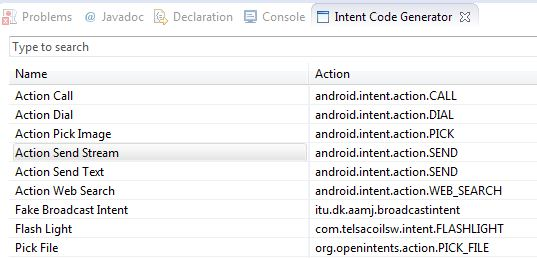
\includegraphics[width=\textwidth]{codegenerator}
  \caption{Final plug-in view}
\end{figure}

{\footnotesize\begin{lstlisting}
Intent ast = new Intent("android.intent.action.SEND");
ast.setType("text/plain");
ast.putExtra("android.intent.extra.TEXT", text);
startActivity(ast);		
\end{lstlisting}}